\chapter{Simspark}
\label{cha:simspark}

In this section you find information about the messages that are sent from the
server to the agent (perceptors) and vice versa (effectors). A description of
the perceptors and effectors can also be found in \cite{SchillingJ} (German), \cite{Lekavy} (Slovak), and to some part in \cite{Vorst06} (concerns the older "spheres" simulation though, so some information is outdated).

%-------------------------------------------------------------------
\section{Perceptors}
\label{sec:perceptors}

Perceptors are used to sense the environment of the agent. They are sent from
the server to each agent and contain agent specific and perceptor specific
information about the environment and the agent itself. There are perceptors
that are available to all kinds of simulations and soccer specific perceptors.

\subsection{General message format}
\label{sec:msgformat}

Messages from and to the server use S-expressions (short for symbolic
expressions) as their basic data structure. The basic idea of
S-expressions is very simple: they are either strings, or lists of
simpler S-expressions.  They are probably best known for their use in
the Lisp family of programming languages where they are used for both
code and data.

An advantage of using S-expressions over other data formats is that it
provides an easy to parse and compact syntax that is to some extent
still readable by humans for debug purposes. It is further easy to add
new sensors to the messages as the parser on the client side can
easily ignore unknown parts.

Messages exchanged between client and server use the default ASCII
character set, i.e. one character is encoded in a single byte. Further
each individual message is prefixed with the length of the payload
message. The length prefix is a 32 bit unsigned integer in network
order, i.e. big endian notation with the most significant bits
transferred first.

% Klaus:do we have noise in perceptors?
% Joschka: only in some so far (e.g. vision); the joint perceptors, gyro, and touch perceptors don't have noise yet (should be on the ToDo list)
\subsection{General Perceptors}
\label{sec:generalperceptors}

The perceptors described in this subsection are available to all types of
simulation. In other words they are not specific to the soccer environment.

\subsubsection{GyroRate Perceptor}
\label{sec:GYR}
The gyro rate perceptor delivers information about the orientation of a body.
Currently only the upper torso contains a gyro perceptor.
The message contains the GYR identifier, the name of the body to which the gyro
perceptor belongs and three rotation angles. These angles describe the
orientation of the body with respect to the global coordinate system.
\begin{itemize}
	\item[Message format:] \texttt{(GYR (n <name>) (rt <x> <y> <z>))}
	\item[Example message:] \texttt{(GYR (n torso) (rt 0.01 0.07 0.46))}
\end{itemize}

%Klaus: To me it is not quite clear what the reference coordinate system is
%Joschka: The coordinate system should be the local coordinate system of the body that the perceptor is attached to. 

\subsubsection{HingeJoint Perceptor}
\label{sec:HJP}
A hinge joint perceptor receives information about the angle of the
correponding single axis hinge joint. It contains the identifier HJ, the name
of the perceptor (see table~\ref{table:perceptorNames}) and
the position angle of the axis. Zero degrees corresponds to straightly allinged bodies. A hinge joint is displayed
in figure \ref{ode:hingejoint}. 

\begin{figure}[htbp]
  \begin{center}
	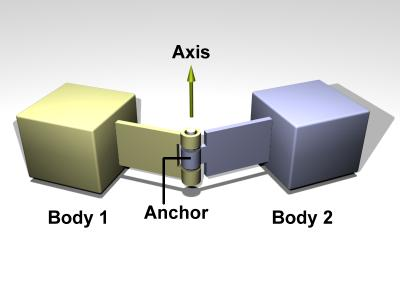
\includegraphics[scale=0.6]{fig/HingeJoint.png}
    \caption{Hinge Joint (\cite{ODEManual})}
    \label{ode:hingejoint}
  \end{center}
\end{figure}

%klaus: What is the zero degree position, is the above correct?
%Joschka: I don't think this is necessarily correct; to my knowledge, the zero position is determined by the orientation and position of the bodies at the time the joint is attached. Is this right?

\begin{itemize}
	\item[Message format:] \texttt{(HJ (n <name>) (ax <ax>))}
	\item[Example message:] \texttt{(HJ (n laj3) (ax -1.02))}
\end{itemize}

\subsubsection{UniversalJoint Perceptor}
\label{sec:UJP}

A universal joint perceptor receives information about the two angles of the
correponding two axis universal joint. It contains the identifier UJ, the name
of the perceptor (see table~\ref{table:perceptorNames}) and the position angles
of the two axis. Zero degrees corresponds to straightly allinged bodies. A universal joint is
displayed in figure \ref{ode:universaljoint}. 
\begin{figure}[htbp]
  \begin{center}
	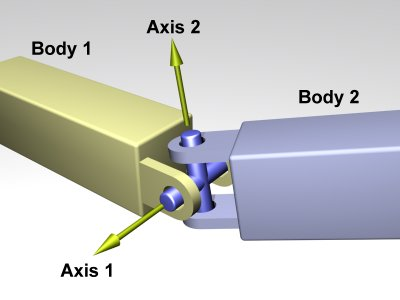
\includegraphics[scale=0.6]{fig/UniversalJoint.png}
    \caption{Universal Joint (\cite{ODEManual})}
    \label{ode:universaljoint}
  \end{center}
\end{figure}
 
\begin{itemize}
	\item[Message format:] \texttt{(UJ (n <name>) (ax1 <ax1>) (ax2 <ax2>))}
	\item[Example message:] \texttt{(UJ (n laj1\_2) (ax1 -1.32) (ax2 2.00))}
\end{itemize}

\subsubsection{Touch Perceptor}
\label{sec:touchperceptor}

This perceptor works like a bumper that is triggered if the agent part
to which it is mounted collides with another simulation object. The
perceptor always reports its own unique name. This allows the use of
more than one touchperceptor per agent. Further the value 0 meaning no
collision detected or 1 meaning collision detected is given.

\begin{itemize}
	\item[Message format:] \texttt{(TCH n <name> val 0|1)}
	\item[Example message:] \texttt{(TCH n bumper val 1)}
\end{itemize}


\subsubsection{ForceResistance Perceptor}
\label{sec:FRP}

This perceptor informs about the force that acts on a body. Currently, it is
available for the left and the right foot (lf, rf).
After FRP and the name of the body it contains two vectors that indicate the
point on the body to which the force applies and the force vector itself.

%klaus: how exactly does this work, what is the unit?
%Joschka: I think Hedayat uses ODE dJointFeedback to get information about the force vector at different contact points and calculates a weighted average of these positions to get the center (weighted by the amount of force at the respective point). The value of the reported force is the total sum of all the force vectors (see also TEXT_INSTEAD_OF_A_MANUAL.txt). I don't know what unit is used though...

%klaus: is this general or soccer specific?
%Joschka: it is a general perceptor

\begin{itemize}
	\item[Message format:] \texttt{(FRP (n <name>) (c <px> <py> <pz>) (f <fx> <fy>
	<fz>))}
	\item[Example message:] \texttt{(FRP (n lf) (c -0.14 0.08 -0.05) (f 1.12 -0.26
	13.07))}
\end{itemize}

\subsubsection{Accelerometer}
This perceptor measures the proper acceleration it experiences
relative to free fall. As a consequence an accelerometer at rest
relative to the Earth's surface will indicate approximately 1 g
upwards. To obtain the acceleration due to motion with respect to the
earth, this ``gravity offset" should be subtracted.
\begin{itemize}
	\item[Message format:] \texttt{(ACC (n <name>) (a <x> <y> <z>))}
	\item[Example message:] \texttt{(ACC (n torso) (a 0.00 0.00 9.81))}
\end{itemize}

\subsection{Soccer Perceptors}
\label{sec:soccerperceptors}

The following perceptors are soccer specific and only available in the soccer
simulation.

\subsubsection{Vision Perceptor}
\label{sec:visionperceptor}

Your robots possess a special omnicam with some smart image processing
software attached :). If using the regular visionperceptor, Robots
have a 360 degrees view. With the RestrictedVisionPerceptor (which
became the default in version 0.5), the view field of the robot is
restricted to 120 degrees (for Nao robot). The direction of the view (pan and tilt) can be
changed with the pantilt effector. The camera can pan to any angle
(the initial 0 degrees pan direction is the direction towards the
opponent side), and tilt around the horizontal plane.

The VisionPerceptor delivers lists of seen objects, where objects are
either others robots, the ball, or markers on the field. Currently
there are 8 markers on the field: one at each corner point of the
field and one at each goal post.

With each sensed object you get (see figure \ref{fig:polarcoordinates}):

\begin{itemize}
  \item The distance between the player and the object.
  \item The angle in the horizontal plane. Zero degree always points to the
opponent goal.
  \item The latitudal angle. Here zero degree means horizontal. 
\end{itemize}

\begin{figure}[htp]
  \centering
  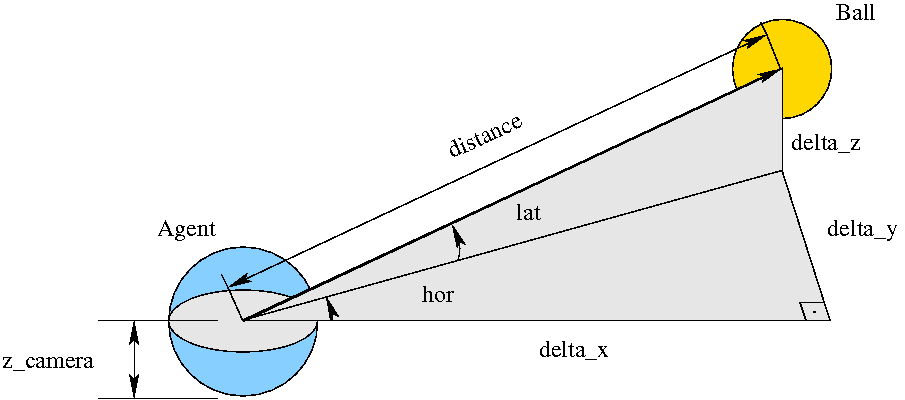
\includegraphics[scale=0.4]{fig/polar_conversion}
  \caption{Polar coordinates as supplied by the 3D Soccer Server \cite{Vorst06}}
  \label{fig:polarcoordinates}
\end{figure}

Contrary to 2D soccer simulation, the vision system does not deliver
object velocities. Objects can be occluded by other objects (this is
not completely implemented yet). All distances and angles are given
relative to the camera position. The camera is currently located at
the center of the robot's torso.

% Klaus: where is it in humanoid league
% Joschka: in the head for most of them, although some robots have an additional camera on the torso pointing down to be able to see the ball if it's right in front of their feet.

The noise parameters of the vision system are as follows:
\begin{itemize}
  \item A small calibration error is added to the camera position. For each
  axis, the error is uniformly distributed between -0.005 m and 0.005 m. The
  error is calculated once and remains constant during the complete match.
  \item Dynamic noise normally distributed around 0.0
  \subitem + distance error:  sigma = 0.0965 (also, distance error is multiplied by distance/100)
  \subitem + angle error (x-y plane): sigma = 0.1225
  \subitem + angle error (latitudal): sigma = 0.1480
\end{itemize}

A vision message is started with See followed by the visible objects.
Possible objects are:
\begin{itemize}
	\item[Flags:] The marker flags on the field corners F1L, F1R, F2L, F2R
	\item[Goalposts:] The goal posts of both goals G1L, G1R, G2L, G2R. Goals and
	flags are located as shown in \ref{fig:pitch}.
	\item[Ball:] The ball B 
	\item[Players:] Players P with additional information \texttt{(team <teamname>)
	(id <playerID>)}
\end{itemize}
\begin{itemize}
	\item[Message format:] \texttt{(See (<name> (pol <distance> <angle1>
	<angle2>)) (P (team <teamname>) (id <playerID>) (pol <distance> <angle1> <angle2>)))}
	\item[Example message:] \texttt{(See (F1L (pol 19.11 111.69 -9.57)) (F2L (pol 
	16.41 -115.88 -11.15)) (F1R (pol 46.53 22.04 -3.92)) (F2R (pol 45.49 -18.74
	-4.00)) (G1L (pol 9.88 139.29 -21.07)) (G2L (pol 8.40 -156.91 -25.00)) (G1R
	(pol 43.56 7.84 -4.68)) (G2R (pol 43.25 -4.10 -4.71)) (B (pol 18.34 4.66
	-9.90)) (P (team RoboLog) (id 1) (pol 37.50 16.15 -0.00)))}
\end{itemize}

% What about the Restricted Vision Perceptor?
% The current soccer bot seems not to use it, still experimental/unsupported?

% Joschka: I'm not sure either. Oliver worked on that, and Yuan had several patches for it last year. Maybe Yuan has the best overview right now? The current Soccerbot doesn't use it.
% Hedayat: Currently Nao robot uses this perceptor.

\subsubsection{GameState Perceptor}
\label{sec:gamestateperceptor}

The GameStatePerceptor contains information of the current play time which
starts from zero at kickoff of either half. It also contains the current game status.
The first percept you get from this perceptor additionally tells you about some
of the game variables, like ball weight and field size.

All other percepts start with GS and contain the current simulation time as a
float value passed in seconds and the playmode. Possible
playmodes are "BeforeKickOff", "KickOff\_Left", "KickOff\_Right",
"PlayOn", "KickIn\_Left", "KickIn\_Right", "corner\_kick\_left",
"corner\_kick\_right", "goal\_kick\_left", "goal\_kick\_right",
"offside\_left", "offside\_right", "GameOver", "Goal\_Left",
"Goal\_Right", "free\_kick\_left", "free\_kick\_right", "unknown". For an
up to date list of all playmodes refer to (./plugin/soccer/soccertypes.h)

\begin{itemize}
	\item[Message format:] \texttt{(GS (t <time>) (pm <playmode>))}
	\item[Example message:] \texttt{(GS (t 0.00) (pm BeforeKickOff))}
\end{itemize}

\subsubsection{AgentState Perceptor}
\label{sec:agentstateperceptor}

The AgentState perceptor gives information about the internal state of
the agent. It reports information about the current battery status and
the temperature of the agent.

\begin{itemize}
	\item[Message format:] \texttt{(AgentState (temp <degree>) (battery <percentile>))}
	\item[Example message:] \texttt{(AgentState (temp 48) (battery 75))}
\end{itemize}

\subsubsection{Hear Perceptor}
\label{sec:hearperceptor}
Agent processes are not allowed to communicate with each other directly, but
agents may exchange messages via the simulation server. For this purpose
agents are equipped with the so-called \emph{hear perceptor}, which serves as
an aural sensor and receives messages shouted by other players. Actually the
underlying model stems from the 2D Soccer Simulation and has been integrated 
in the 3D~simulator since server version~0.4. Percepts have the following format:
\begin{itemize}
	\item[Message format:] \texttt{(hear <time>	'self'|<direction> <message>)} 
	\item[Example message:]	\texttt{(hear 12.3 self ``helloworld'')}
\end{itemize}
The value of $time$ is a real number and reflects the time when the given
message was heard. ${S}ource$ is either the relative direction in degrees
where the sound was located, or {\tt self} if the player has a statement by
his own. $Message$ may consist of characters from the ASCII printing character
subset \mbox{$[{\tt 0x20}, {\tt 0x7E]}$}, among which the alphanumerical
symbols and mathematical operators can be found for example. Three characters
from this range are, however, excluded: the {\it white space} character
($\sqcup$) and the normal brackets {\tt(} and {\tt )}.

The hear perceptor comes up with some restrictions:
\begin{enumerate}
	\item Messages are restricted to a \emph{maximal length} (currently 20 bytes).
	\item Messages shouted from beyond a \emph{maximal distance} (currently $50.0$ meters) cannot be heard.
	\item The \emph{number of messages} which can be heard at the same time is
	bounded: Each player has the maximal capacity of one heard message by a
	specific team every two sensor cycles (thus every $0.4$ seconds per team).
	There are separately tracked capacities for both teams, because teams should
	not be able to block the hear perceptors of their opponents by shouting
	permanently. If more messages from players of one team arrive, they are
	processed in the order of arrival; the remaining messages are simply not
	heard.\\ Messages shouted by oneself, though, can always be noticed
	\cite{Vorst06}.
\end{enumerate}


%-------------------------------------------------------------------
\section{Effectors/Actuators}
\label{sec:effectors}

Effectors are used to act within the simulation. They are sent to the server
to change the game state accordingly. There are effectors that are available to
all kinds of simulations and soccer specific effectors.

%Klaus: do we have noise in effectors?
% Joschka: only in the old kick effector (we need noise models though, should be a ToDo)

%Klaus: What are the minimal/maximal values to pass? What happens in case of
% errors
% Joschka: Good question ;-) For the joint effectors, you supply angles in degrees, there should be no problem. For anything else, I'm not sure.

\subsection{General Effectors}
\label{sec:generaleffectors}

The effectors described in this subsection are available to all types of
simulation. In other words they are not specific to the soccer environment.

\subsubsection{Create Effector}
\label{sec:createeffector}

When an agent initially connects to the server it is invisible and
cannot take affect a simulation in any meaningful way. It only
possesses a so called CreateEffector.

An agent uses this effector to advice the server to construct it
according to a scene description file it passes as a parameter. This
file is used to construct the physical representation and all further
effectors and preceptors.
\begin{itemize}
	\item[Message format:] \texttt{(scene  <filename>)}
	\item[Example message:] \texttt{(scene rsg/agent/nao/nao.rsg)}
\end{itemize}

After the agent representation is constructed in the server the agent
should do further simulation specific setup. For example in the soccer
simulation each agent is required to register to a team and acquire a
unique player number. For these tasks usually a special effector like
the SoccerInitEffector is used.

\subsubsection{HingeJoint Effector}
\label{sec:HJE}

Effector for all axis with a single degree of freedom.
The first parameter is the name of the axis. Table ??? shows a list of all
available hinge joints. The second parameter contains the change in angle of
the joint.
\begin{itemize}
	\item[Message format:] \texttt{(<name> <ax>)}
	\item[Example message:] \texttt{(lae3 5.3)}
\end{itemize}

\subsubsection{UniversalJoint Effector}
\label{sec:UJE}

Effector for all axis with a two degrees of freedom.
The first parameter is the name of the axis. Table ??? shows a list of all
available hinge joints
The second and third parameter contain the change in angle of the two joints.
The order of the joints is the same as in the name.
\begin{itemize}
	\item[Message format:] \texttt{(<name> <ax1> <ax2>)}
	\item[Example message:] \texttt{(lae1\_2 -2.3 1.2)}
\end{itemize}

\subsection{Soccer Effectors}
\label{sec:soccereffectors}

The following effectors are soccer specific and only available in the soccer
simulation.

\subsubsection{Init Effector}
\label{sec:initeffector}

The init command is sent once for each agent after the create effector sent the
scene command. It registers this agent as a member of the passed team with the passed number.
All players of one team have to use the same teamname and different numbers.
If an agent sends 0 as playernumber, the number is assigned automatically by
the server to the next free number. The maximum amount of teams is two, the
maximal amount of players is currently four.
The side on which a team starts to play depends on which team connected
first.
\begin{itemize}
	\item[Message format:] \texttt{(init (unum <playernumber>)(teamname
	<yourteamname>))}
	\item[Example message:] \texttt{(init (unum 1)(teamname FHO))}
\end{itemize}

\subsubsection{Beam Effector}
\label{sec:beameffector}

The beam effector allows a player to position itself on the field before the
game starts. The x and y coordinates define the position on the field with
respect to the coordinate system of figure ???. The rot value allows to define
the rotation angle of the player. Zero degrees points to positive x axis, 90
degrees to positive y axis.
\begin{itemize}
	\item[Message format:] \texttt{(beam <x> <y> <rot>)}
	\item[Example message:] \texttt{(beam 10.0 -10.0 0.0)}
\end{itemize}

\subsubsection{Say Effector}
\label{sec:sayeffector}

%klaus: is this old version only?
%Joschka: no, the Soccerbot has a say effector in the current version. It is restricted to 20 bytes msgs.
%description in TEXT_INSTEAD_... and Philipp Vorst's thesis
The \emph{say effector} permits communication among agents by broadcasting
messages. In order to say something, the following command has to be employed:
\begin{itemize}
	\item[Message format:] \texttt{(say <message>)}
	\item[Example message:] \texttt{(say ``helloworld'')}
\end{itemize}
$Message$ may consist of 20 characters, which may be taken from the ASCII 
printing character subset $[{\tt 0x20}, {\tt 0x7E]}$ except the {\it white
space}  character ($\sqcup$) and the normal brackets {\tt(} and {\tt )}. 
For details and restrictions please see Section~\ref{sec:hearperceptor}, about
the \emph{hear perceptor}, the dual sensor to this actuator.

\subsection{Older Version Effectors}
\label{sec:olderversioneffectors}

The effectors in this subsection have been available in older versions of the
simulation and are now no longer available

\subsubsection{Drive Effector}
\label{sec:driveeffector}

To use the omnidrive of the agent, you have to use the so called
"DriveEffector", which takes a cartesian vector (x y z) with a maximum
length of 100 units. The x-coordinate points towards the opponents
team side of the field, z points up. With the DriveEffector, you set a
kind of motor force, i.e. if you want to drive full speed for a while,
it is sufficient to use the DriveEffector *once*. The force you set is
applied at each simulator step until you change it again. The
DriveEffector works reliable, there is a small error for forces along
each axis (each up to 2\% of the applied force). The error is normally
distributed around 0.0.

Using the omnidrive consumes battery. You get to know of battery
states by reading the AgentStatePerceptor. If the battery is empty,
the omnidrive will stop working. It is also possible to push away
other robots. Using this feature to push away opponents is discouraged
:).

\begin{itemize}
	\item[Message format:] \texttt{(drive <x> <y> <z>)}
	\item[Example message:] \texttt{(drive 20.0 50.0 0.0)}
\end{itemize}

\subsubsection{Kick Effector}
\label{sec:kickeffector}

To move the ball, you have the option of simply using the robots to
push the ball into a desired direction, or you can use the
kickeffector to kick the ball. Originally, we did not intend to create
an artificial kickeffector. However, to make use of the 3rd dimension,
this was the easiest way. It is intended to remove this kind of kick
effector in future versions (not this years' competition) in favor of
a real physical device.

The kickeffector can accelerate the ball radially away from the robot
body. The kickeffector takes an angle as first argument. This is the
latitudal angle (in degrees) for accelerating the ball. It is
restricted to a number between 0 and 50. The second argument indicates
the kicking power and this is a number between 0 and 100. It is
interpreted as the percentile of the maximum available power. The
kickeffector adds a force and a torque to the ball. This happens over
a fixed number of simulation steps. Currently 10 cycles are used. This
corresponds to 1/10s simulation time. To kick the ball, the ball has
to be very close to the robot, i.e. it has to be within the so called
kickable margin of the player. Currently 0.04m are configured.

You cannot change the kicking angle in the horizontal plane. This
means that you have to move the robot so that it can kick into the
desired direction. Right now, the kickeffector is not very strong,
because something like an offside rule is missing. It should also not
be possible to move other robots by kicking the ball against them
anymore. (at least not very much :) Like the DriveEffector, the
kickeffector does only work if the robot touches the soccer field.

The kickeffector noise has the following parameters: 
\begin{itemize}
\item The angle error in the x-y plane is quite low and normally distributed
around 0.0 with sigma = 0.02.
\item The latitudal angle error is normally distributed around 0.0. This
angle error is low with sigma = 0.9 at both extreme positions, i.e. 0
and at 50 degrees. Towards the middle of the range the angle error
gets higher with sigma up to 4.5.
\item The kick power error is normally distributed around 0.0 with sigma =
0.4
\end{itemize}

\begin{itemize}
	\item[Message format:] \texttt{(kick <angle> <power>)}
	\item[Example message:] \texttt{(kick 20.0 80.0)}
\end{itemize}

% illustration from Philipp's thesis here?

\subsubsection{Catch Effector}
\label{sec:catcheffector}

The goalie (agent number 1) is the only player with the ability to
catch a ball. The goalie can catch the ball in play mode 'playe\_on',
if the ball is inside the penalty area and close to the robot, i.e. it
has to be within the so called catch margin of the player. The current
value of catch margin is 2 meters.

The catcheffector puts the ball in front of the goalie on the ground
and moves players away that are closer than 2 meters to the goalie by
5 meters.

\begin{itemize}
	\item[Message format:] \texttt{(catch)}
	\item[Example message:] \texttt{(catch)}
\end{itemize}

% illustration from Philipp's thesis here?

%----------------------------------------------------------------------
\section{Simulation Update Loop}

SimSpark implements a simple internal event model that immediately
executes every action received from an agent. It does not try to
compensate any network latency or compensate for different computing
resources available to the connected agents.

A consequence is that SimSpark currently does not guarantee that
events are reproducible. This means repeated simulations may have a
different outcome, depending on network delays or load variations on
the machines hosting the agents and the server.

A benefit of the simple structure however are speed gains that make it
interesting for machine learning tasks as in these setups an often
large number of different agent and simulation configurations are
repeatedly tested.

Further the SimSpark main loop is highly customizable as it is
entirely build upon plugins we call simcontrol nodes. Simcontrol nodes
are registered to the simulation server. They act in response to
control events. The simulation server repeatedly generates these as it
executes an abstracted the main loop.

The event types are an 'init' event once when the simulation server
starts and a 'done' event on shutdown. The main then loop cycles
repeatedly through the 'start cycle', 'sense agent', 'act agent' and
'end cycle' events.

Apart from generating control events the simulation server advances
the simulation time passed in the last cycle. Depending on its
configuration it either does this in discrete time quanta or in one
single step.

A simcontrol node further can take responsibility for the time
measurement, for example to synchronize the simulation time with the
real time used to render the scene.  Otherwise the simulation is
stepped a fixed time step as often as possible.

In this way all management tasks are implemented as plugins to the
simulation server. This involves the agent management, monitor
management, rendering, mouse and keyboard input and network code.

This setup allows us to configure the simulation at runtime as either
a monolithic application that does both simulation and rendering or as
a dedicated simulation server that defers rendering to a remote
monitor application.

\subsection{Single-threaded Timer}

In the singled-threaded mode, the main loop cycles repeatedly through
the `start cycle', `sense agent', `act agent' and `end cycle' events(
see \autoref{fig:single-thread-sd}). There are two noticeable details:
\begin{itemize}
\item Each cycle duration is 20ms, if the simulation is fast than real
  time, it will wait; otherwise, if the simulation is very slow, it
  will run many physics updates once without interaction with agents.
  If the simulation is very slow, it will give up to catch up the real
  time and print warning. So you may have problem while the computer
  is not fast enough.
\item The `act agent' event is followed after `sense agent', the
  action which the agent send according to $n^{th}$ cycle will be
  realized in the $(n+1)^{th}$ cycle, i.e. the action has been delayed
  one cycle. See for \autoref{fig:synchronization} explanation.
\end{itemize}

\begin{figure}[htp]
  \centering
  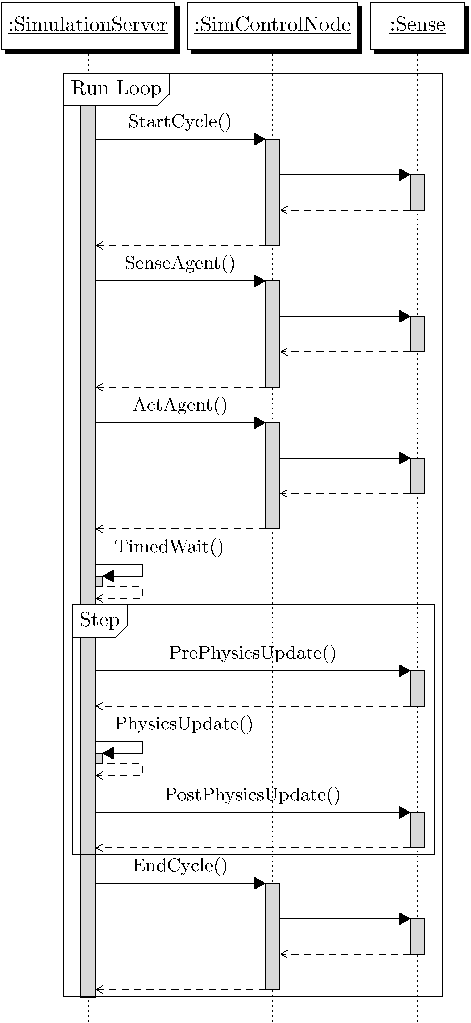
\includegraphics[height=0.6\textheight]{fig/serverSingleThreadLoop}
  \caption{Single-threaded loop UML sequence diagram}
  \label{fig:single-thread-sd}
\end{figure}

\begin{figure}[htp]
  \centering
  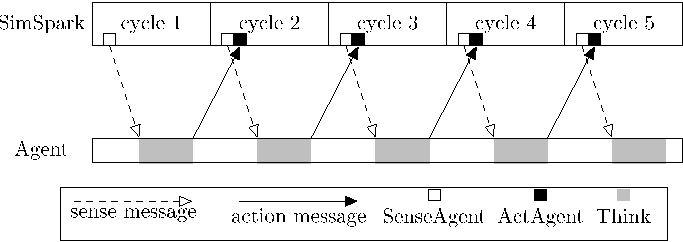
\includegraphics[width=0.8\textwidth]{fig/synchronization}
  \caption{Synchronization between SimSpark and agent}
  \label{fig:synchronization}
\end{figure}

\subsection{Multi-threaded Timer}
In modern time, computers have more than one CPU or dual cores in one
CPU. This improve the performance greatly, but only the multi-threaded
program can benefit. SimSpark has an experimental multi-threaded
running loop, it can be switched on simply by change the
\texttt{simulationServer.setMultiThreads(false)} to
\texttt{simulationServer.setMultiThreads(true)} in the
\texttt{spark.rb} file.

The implementation of multi-threaded loop is based on two conditions.
First, every SimControlNode response for different parts of the
simulation, they perform one by one in the singled-threaded mode, but
they can run in parallel. Second, there is a active scene which stores
the whole simulation data in a tree. The physics engine and
SimControlNode interact through the active scene. As we know, the
physics computation is the most time-consuming, and the physics engine
does not need to access the active scene during physics computation.
So the physics computation and SimControlNodes can run in parallel. At
last, we get the multi-threaded simulation loop as
\autoref{fig:multi-thread-sd}. Note that the agent's action are also
delayed one cycle in the multi-threaded loop.
\begin{figure}[htp]
  \centering
  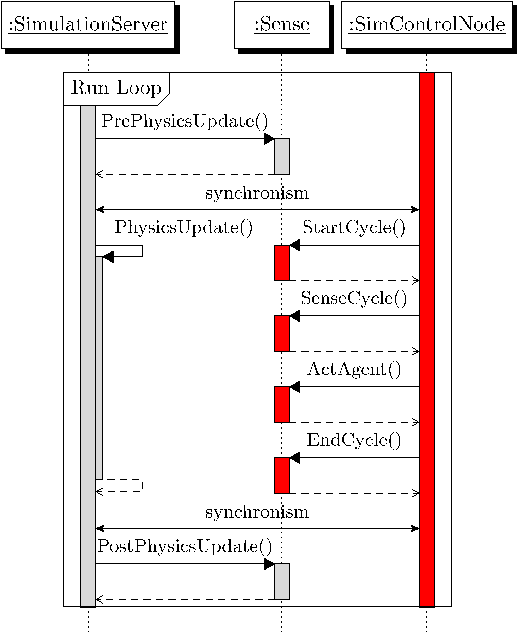
\includegraphics[height=0.5\textheight]{fig/serverMultiThreadLoop}
  \caption{Multi-threaded loop UML sequence diagram, note that
    each SimControlNode runs in separated thread.}
  \label{fig:multi-thread-sd}
\end{figure}

%----------------------------------------------------------------------
%\section{Setup Scripts}

%\textbf{TODO:}

%\begin{itemize}
%\item describe purpose of scripts in \~/.rcssserver3d/
%\item kerosin.rb for rendering configuration of simspark
%\end{itemize}

%%% Local Variables: 
%%% mode: latex
%%% TeX-master: "user-manual"
%%% End: 
